\documentclass[twocolumn]{aastex62}

\newcommand{\vdag}{(v)^\dagger}
\newcommand\aastex{AAS\TeX}
\newcommand\latex{La\TeX}

\newcommand{\project}[1]{\textsl{#1}}
\newcommand{\JWST}{\project{JWST}}
\newcommand{\HST}{\project{HST}}
\newcommand{\Spitzer}{\project{Spitzer}}
\newcommand{\Kepler}{\project{Kepler}}

\submitjournal{AJ}

\shorttitle{Molecular Dissociation in Ultra-Hot Jupiter WASP-33b}
\shortauthors{Kreidberg et al.}

\begin{document}

\title{Evidence for Molecular Dissociation in the Dayside Atmosphere of the Ultra-Hot Jupiter WASP-33b}

\author{Laura Kreidberg}
\affiliation{Harvard-Smithsonian Center for Astrophysics, 60 Garden Street, Cambridge, MA 02138}
\affiliation{Harvard Society of Fellows, 78 Mount Auburn Street, Cambridge, MA 02138}

\begin{abstract}
WASP-33b is hot.
\end{abstract}

\keywords{planets and satellites: individual (WASP-33b), planets and satellites: atmospheres}

\section{Introduction} \label{sec:intro}
Ultra-hot Jupiters (with equilibrium temperatures $T_\mathrm{eq} > 2500$ K) are so highly irradiated that their atmospheric physics and chemistry are on the boundary between planets and stars. Consensus is growing that many molecules dissociate in the hot dayside atmosphere, only to recombine on the cooler nightside \citep{arcangeli18, parmentier18, lothringer18}. 

Most ultra-hot Jupiters have blackbody-like near-infrared emission spectra that are consistent with a single photospheric temperature \citep{arcangeli18, kreidberg18b, mansfield18}.
Previous observations of WASP-33b presented a puzzling outlier (list all).

WASP-33b, \citep[a gas giant in a 1.22 day orbit around a $\delta$ Scuti star][]{cameron10} 

\section{Observations} \label{sec:observations}
We observed WASP-33b with the Wide Field Camera 3 (WFC3) instrument on \HST\ for GO Program 15109 (PI: L. Kreidberg). The observations were obtained over five consecutive orbits of the telescope. We began each orbit with a direct image of the star with the F139M filter (used as a zero-point for wavelength calibration). Subsequent exposures used the G102 grism to obtain time-series spectra over the wavelength range $0.8 - 1.1\,\mu$m. For the spectroscopy, we used ``round-trip" spatial scanning mode, which scans the telescope in the spatial direction back and forth across the detector. This mode enables long exposures for bright targets that quickly saturate in traditional staring mode \citep[compare][]{berta12, kreidberg14a}.  The G102 exposures used the \texttt{SPARS10} readout pattern with \texttt{NSAMP} $= 9$ (for a total exposure time of 83 s). The scan rate was 0.343 arcsec/sec scan rate. This setup yielded a scan height of 170 pixels and maximum per pixel counts to below 30k electrons. 

\section{Data Reduction and Analysis} \label{sec:reduction}

\subsection{Gaussian Process Model for Stellar Oscillations}
Previous analysis of Spitzer phase curves for WASP-33b successfully used a Gaussian process (GP) to model the stellar oscillations \citep{zhang17}. We explored using the same model as \cite{zhang17}, implemented with the \texttt{celerite} package \citep{foremanmackey17}. Briefly, the model has the same power spectrum as a damped simple harmonic oscillator, and a jitter term is added to the diagonal of the covariance matrix to model the photon noise.  We tested this model on the G102 broadband light curve, and found that it significantly improved the fit quality. By replacing the sinusoid model for the stellar oscillations with a GP, we improved the best fit rms to 53 ppm from FIXME ppm.

The improvement to the fit quality was encouraging; however, we found that the GP was so flexible that it could entirely replace the secondary eclipse model. To illustrate, Figure~\ref{fig:GP} shows the best fit for two cases: one that includes a secondary eclipse in addition to the GP and instrument systematics model, and another with the GP and instrument systematics alone. Both cases have identical residuals (53 ppm rms), indicating that the GP can entirely replace the secondary eclipse model. This finding was confirmed from an MCMC fit to the light curve, which yielded an eclipse depth of $796 \pm 357$ ppm (consistent with zero).  We therefore concluded that GPs are not the best model for this data set, and that more data points and/or better time sampling are needed to precisely determine the morphology of the stellar oscillations.

\begin{figure*}
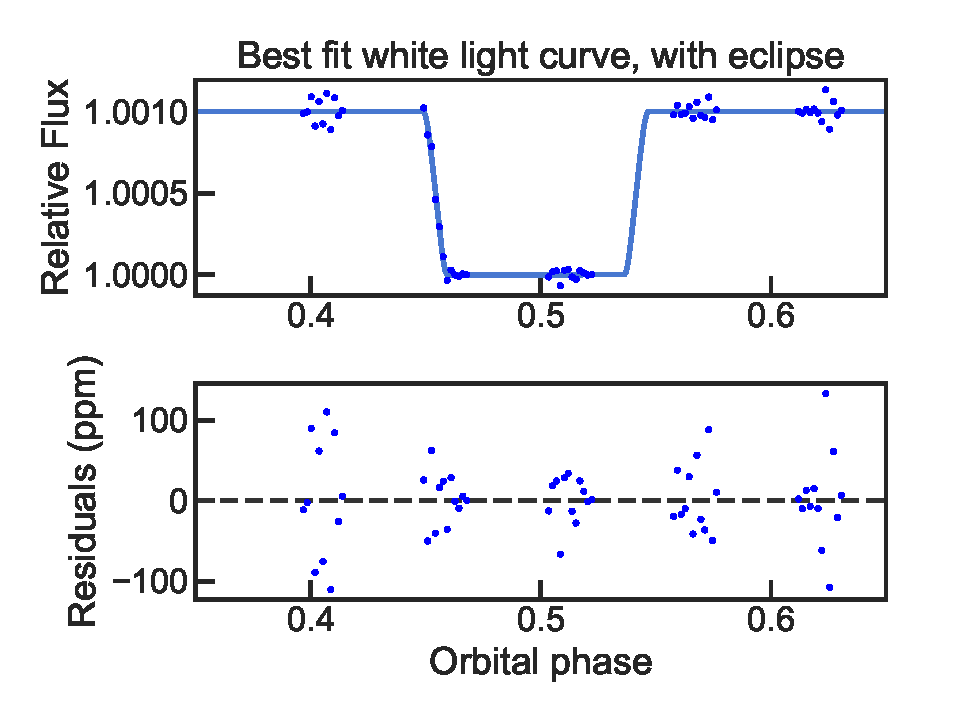
\includegraphics[width = 0.5 \textwidth]{figures/eclipse.pdf}
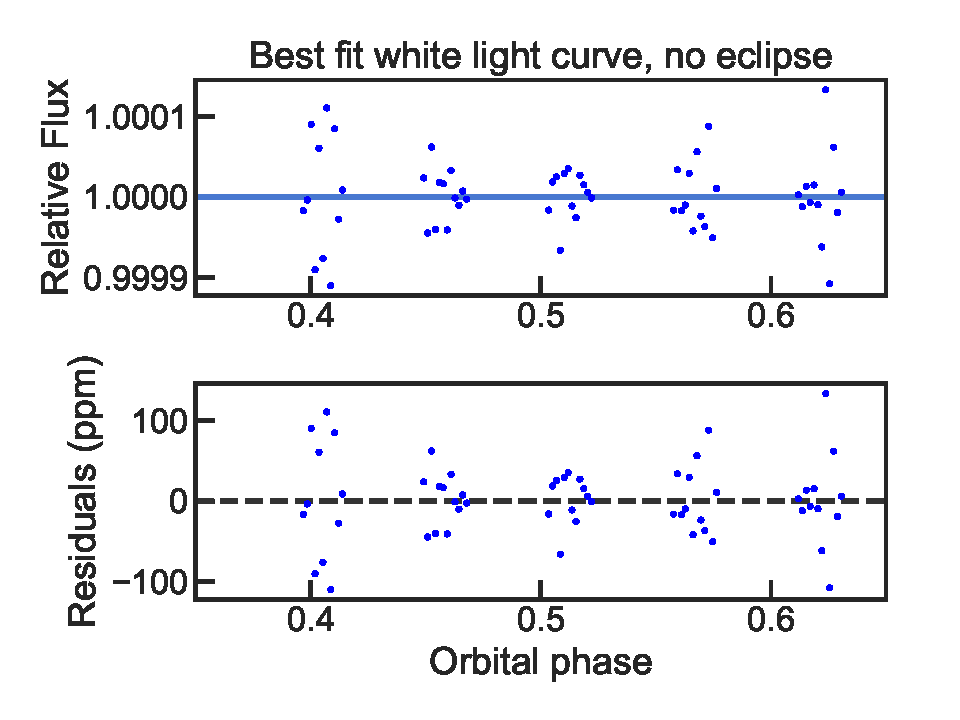
\includegraphics[width = 0.5 \textwidth]{figures/no_eclipse.pdf}
\caption{Top: best fit, broadband G102 light curves (points) for a model that includes an eclipse (left), versus no eclipse (right). The data are normalized (i.e., the light curves are divided by the instrument systematics model and a GP fit to the stellar oscillations). Bottom: residuals to the best fit models. The residuals are nearly identical for the two cases, indicating that the GP is flexible enough to simutaneously model the secondary eclipse and the stellar oscillations for this data set.} 
\label{fig:GP}
\end{figure*}

\subsection{Comparison with \cite{haynes15}}
FIXME: make sure to reach out to A. Mandell with a draft of this!
We also reanalyzed 

Our analysis differs from \cite{haynes15} in two principle ways. One is that we use different orbital parameters for the system. \cite{haynes15} do not report their eclipse times; however, by inspection of their best fit light curve (Figure FIXME), ingress begins earlier/later. We use the precise orbital parameters from \cite{zhang17}.

Another key difference from \cite{haynes15} is that we do not assume the instrument systematics are constant with wavelength. WFC3 systematic trends are known to depend on the count rate \cite{zhou17}, so we allowed the systematics parameters to vary in each spectroscopic light curve fit.  Figure FIXME shows the params.


\subsection{Companion Star}

\acknowledgments
Dan FM. Thomas Beatty -- albedo spectrum! Jayne Birkby - putting me in touch with Josh.

\bibliographystyle{aasjournal}
\bibliography{ms.bib}

\end{document}

% End of file `sample62.tex'.
